\documentclass[12pt]{article}
\usepackage[a4paper,margin=1in]{geometry}
\usepackage{amsmath,amssymb}
\usepackage{graphicx}
\usepackage{siunitx}
\sisetup{per-mode=symbol}
\usepackage{gvv}

\title{Matrix 2.6.24}
\author{ai25btech11015 -- M Sai Rithik}
\date{}

\begin{document}
\maketitle

\section*{Question (2.6.24)}
Find the area of the parallelogram formed by the vectors
\[
\Vec{a} = 3\hat{i} + \hat{j} + 4\hat{k}, \qquad
\Vec{b} = \hat{i} - \hat{j} + \hat{k}.
\]
Use the cross product definition.

\section*{Solution}

\begin{enumerate}
\item Let
\begin{align}
\Vec{A} &= \myvec{a_1 \\ a_2 \\ a_3}, \\
\Vec{B} &= \myvec{b_1 \\ b_2 \\ b_3},
\end{align}
and define the sub-vectors
\begin{align}
\Vec{A}_{ij} = \myvec{a_i \\ a_j}, \qquad
\Vec{B}_{ij} = \myvec{b_i \\ b_j}.
\end{align}

\item The cross product of $\Vec{A}$ and $\Vec{B}$ is defined as
\begin{align}
\Vec{A}\times\Vec{B} =
\myvec{
  \mydet{\Vec{A}_{23} & \Vec{B}_{23}} \\
  \mydet{\Vec{A}_{31} & \Vec{B}_{31}} \\
  \mydet{\Vec{A}_{12} & \Vec{B}_{12}}
}.
\end{align}

\item For the given vectors
\begin{align}
\Vec{a} = \myvec{3 \\ 1 \\ 4}, \qquad
\Vec{b} = \myvec{1 \\ -1 \\ 1}.
\end{align}

\item Substituting into the definition:
\begin{align}
\Vec{a}\times\Vec{b} &=
\myvec{
\mydet{\myvec{1 \\ 4} & \myvec{-1 \\ 1}} \\
\mydet{\myvec{4 \\ 3} & \myvec{1 \\ 1}} \\
\mydet{\myvec{3 \\ 1} & \myvec{1 \\ -1}}
} \\[1ex]
&= \myvec{
(1)(1) - (4)(-1) \\
(4)(1) - (3)(1) \\
(3)(-1) - (1)(1)
} \\[1ex]
&= \myvec{5 \\ 1 \\ -4}.
\end{align}

\item Area of the parallelogram is
\begin{align}
\text{Area} = \|\Vec{a}\times\Vec{b}\|
= \sqrt{5^2 + 1^2 + (-4)^2}
= \sqrt{42}.
\end{align}
\end{enumerate}

\section*{Final Answer}
\[
\boxed{\text{Area} = \sqrt{42}}
\]

\begin{figure}[h!]
\centering
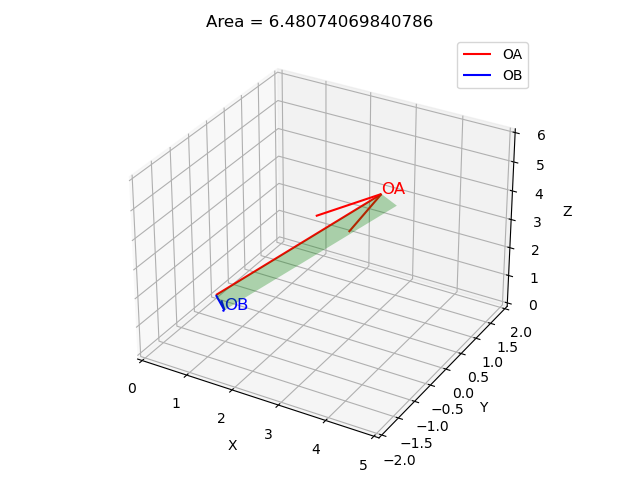
\includegraphics[width=0.6\linewidth]{figs/fig.png}
\caption{Parallelogram spanned by $\Vec{a}$ and $\Vec{b}$.}
\end{figure}

\end{document}
